\documentclass[report.tex]{subfiles}
\begin{document}

\chapter{Excercise 1A: single mass}


\begin{figure}[h!]
  \centering
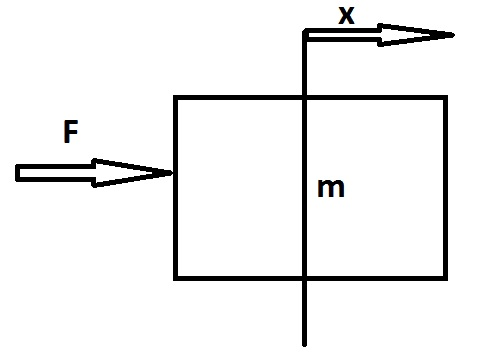
\includegraphics[width=\textwidth,height=\textheight,keepaspectratio]{1A3_system}
\caption{Bode plot of the single mass system}
\end{figure}

The single mass system is shown as free body diagram in figure~\ref{fig:1A3_system}. Specified properties are: 
$ m = 0.1 $

The frequency plot given by diet is: \\

\begin{figure}[h!]
  \centering
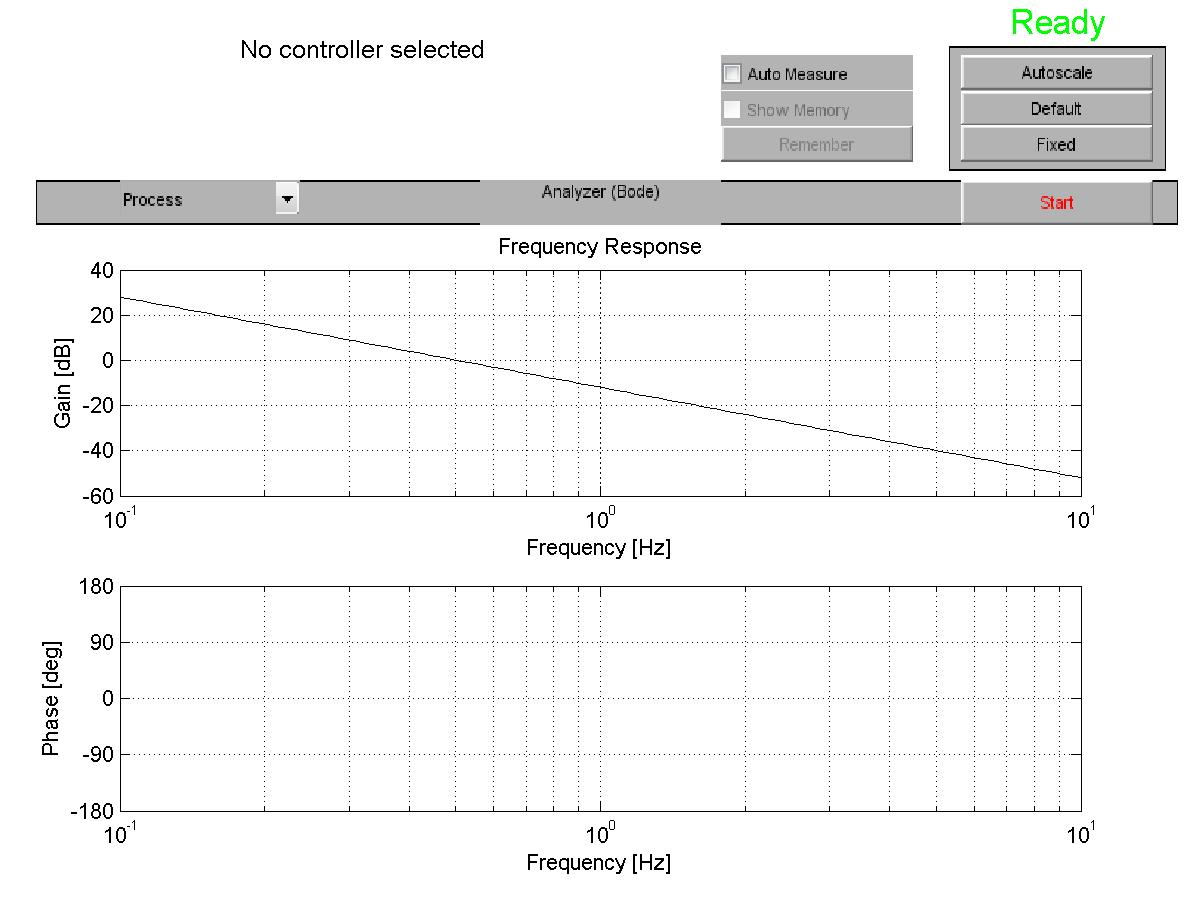
\includegraphics[width=\textwidth,height=\textheight,keepaspectratio]{1A3a_bode}
\caption{Bode plot of the single mass system}
\end{figure}

From this plot it can be concluded that the gain 1 frequency is: INSERT FREQUENCY

The differential equation for this systems is defined as

\begin{equation}
\label{eq:ex1a_diff}
m\ddot{x} = F
\end{equation}

This results in a transfer function by combining following equation
\begin{equation}
\label{eq:ex1a_tf_mass_2}
mX(S)s^2 = F(s) => H(S) = \frac{X(S)}{F(S)} = \frac{1}{ms^2}
\end{equation}

To determine the frequency where the gain is 1 equation~\ref{eq:ex1a_tf_freq_1} needs to be solved. 
\begin{equation}
\label{eq:ex1a_tf_freq_1}
|H(jw)| = |\frac{1}{m(j\omega)^2}| = \frac{1}{m\omega^2} = 1
\end{equation}

The following frequency will be:
\begin{equation}
\label{eq:ex1a_tf_freq_2}
\omega = 2\pi f = sqrt(\frac{1}{m}) => f = \frac{1}{2\pi}sqrt(\frac{1}{m}) 
\end{equation}

This system needs to be stabilized. For this a controller with the form $C(s) = k_p + k_v s$ is used.
The resulting bode plot is showed in figure~\ref{fig:1A4_bode}

\begin{figure}[h!]
  \centering
    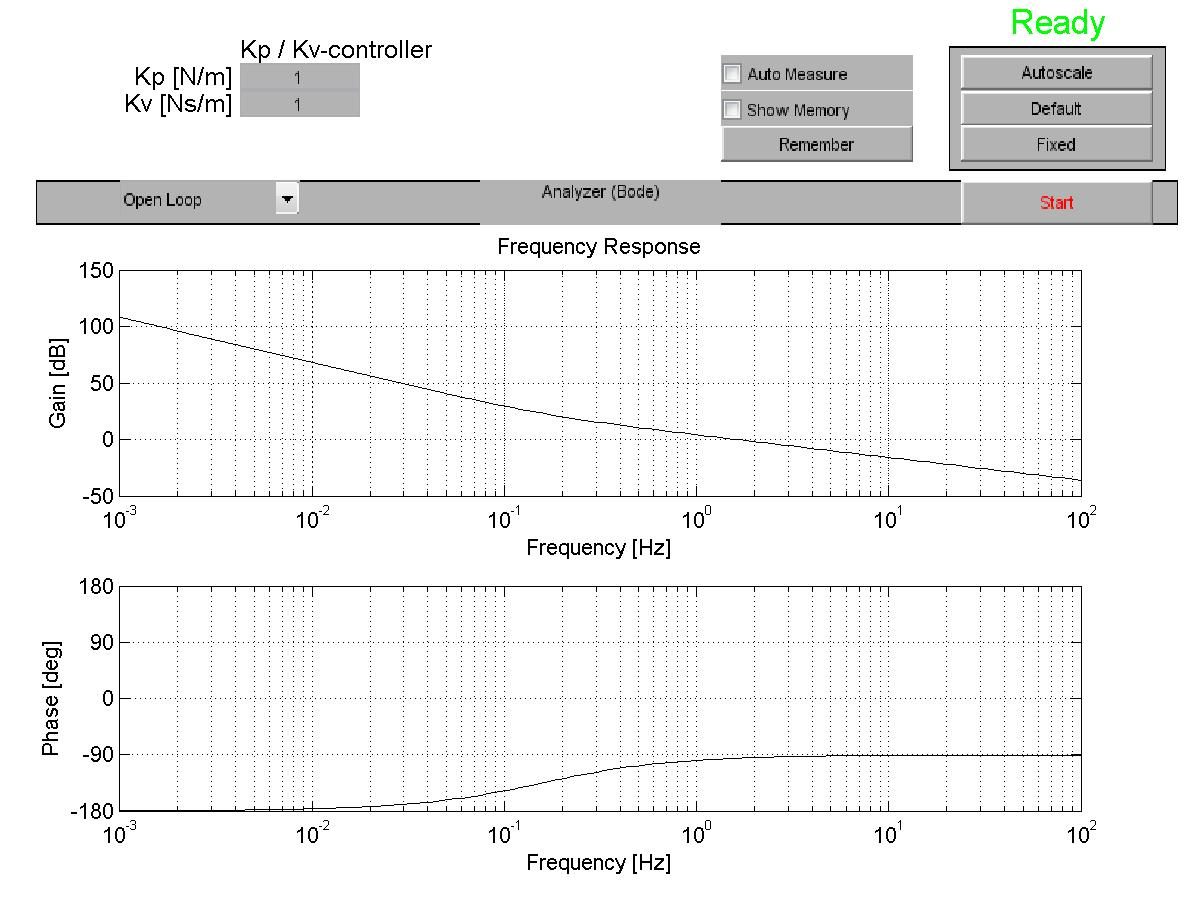
\includegraphics[width=\textwidth,height=\textheight,keepaspectratio]{1A4_bode}
 	\caption{Bode plot of the single mass system with controller $C(S)$}
  \label{fig:1A4_bode}
\end{figure}
To investigate the effect of varying the controller parameters $K_p$ and $K_v$ another 2 bode plots, figure figure~\ref{fig:1A4_bode_k} and figure~\ref{fig:1A4_bode_v}, have been created
\begin{figure}[h!]
  \centering
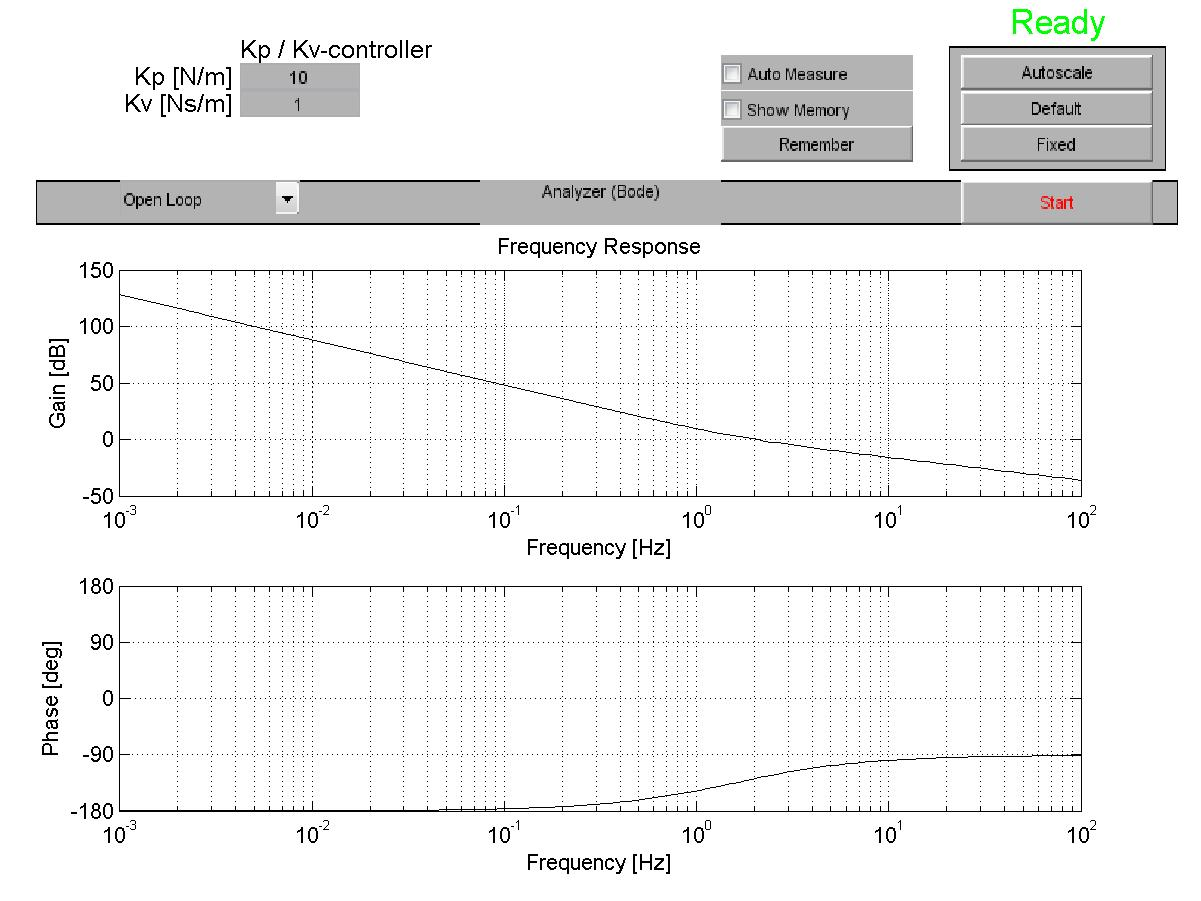
\includegraphics[width=\textwidth,height=\textheight,keepaspectratio]{1A4_bode_k}
\caption{Bode plot of the single mass system with controller $C(S)$ with higher $k_p = 10, k_v
 = 1$}
\label{fig:1A4_bode_k}
\end{figure}

\begin{figure}[h!]
  \centering
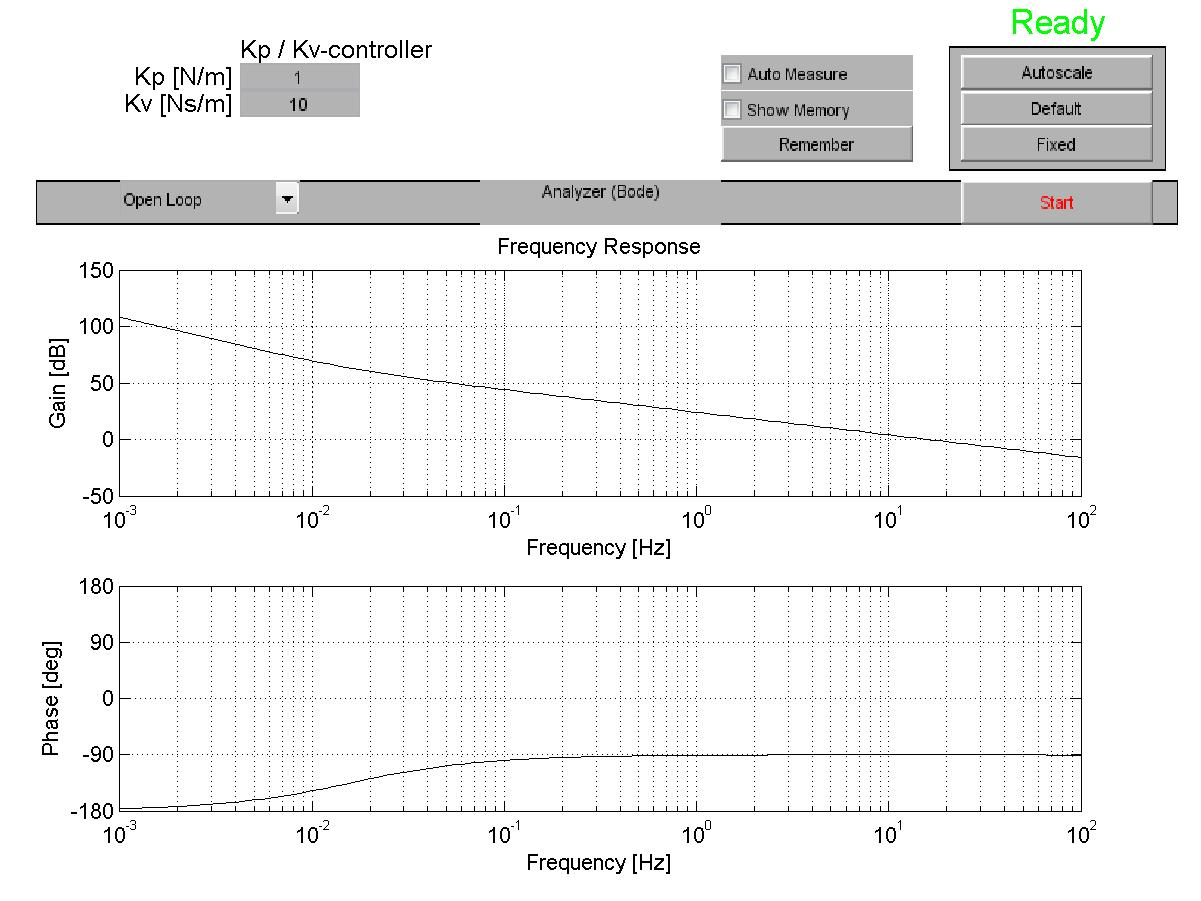
\includegraphics[width=\textwidth,height=\textheight,keepaspectratio]{1A4_bode_v}
\caption{Bode plot of the single mass system with controller $C(S)$ with higher $k_p = 1, k_v = 10$}
\label{fig:1A4_bode_v}
\end{figure}

Effecten:

Zero verplaatst naar hogere frequenties bij hogere k_p

Kp verhoogt de totale gain van bij verhoging

Kv verplaatst de zero richting de hogere frequenties
Tegelijkertijd wordt ook de cross over frequentie 
\end{document}





